\section{Biblioteka tinyUSB}
    \begin{frame}{tinyUSB}
        \begin{itemize}
            \item aktywnie wspierana
            \item wspiera 67 rodzin procesorów różnych producentów
            \item implementuje stosy USB host/device
            \item implementuje różne "deskryptory"
            \item stosunkowo proste użycie
            \item example są, jest ich dużo, ale są mało czytelne
        \end{itemize}
        \begin{figure}[h]
            \centering
            
\includegraphics[width=0.5\textwidth]{images/tinyusb.png}
        \end{figure}
    \end{frame}

    \begin{frame}{Przegląd możliwości}
        \begin{itemize}
            \item Audio Class 1.0/2.0 (UAC1/UAC2)
            \item Bluetooth Host Controller Interface (BTH HCI)
            \item \textbf{Communication Device Class (CDC)}
            \item Device Firmware Update (DFU): DFU mode (WIP) and Runtime
            \item Human Interface Device (HID): Generic (In & Out), Keyboard, Mouse, Gamepad
            \item Printer class
            \item \textbf{Mass Storage Class (MSC): with multiple LUNs}
            \item Musical Instrument Digital Interface (MIDI)
            \item Media Transfer Protocol (MTP/PTP)
            \item \textbf{Network with RNDIS, Ethernet Control Model (ECM), Network Control Model (NCM)}
            \item Test and Measurement Class (USBTMC)
        \end{itemize}
    \end{frame}

    \begin{frame}{Użycie}{CubeMX}
        \begin{figure}[h]
            \centering
            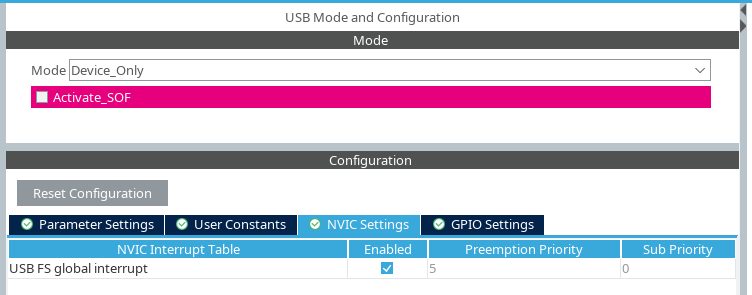
\includegraphics[width=0.9\textwidth]{images/tinyusb_cubemx1.png}
        \end{figure}
    \end{frame}

    \begin{frame}{Użycie}{CubeMX c.d}
        \begin{figure}[h]
            \centering
            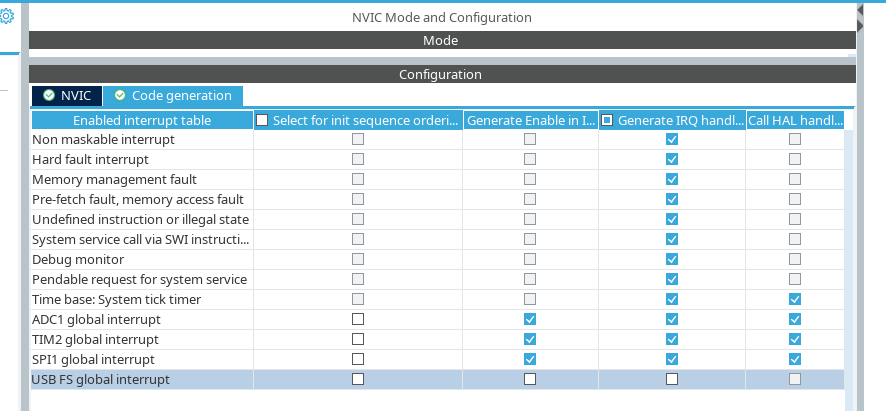
\includegraphics[width=0.9\textwidth]{images/tinyusb_cubemx2.png}
        \end{figure}
    \end{frame}

    \begin{frame}{Użycie}{kod}
        \begin{figure}[h]
            \centering
            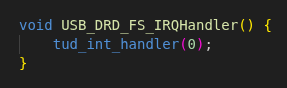
\includegraphics[width=0.8\textwidth]{images/tinyusb_isr.png}
        \end{figure}
            \begin{figure}[h]
            \centering
            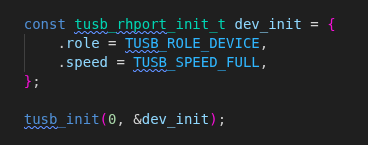
\includegraphics[width=0.8\textwidth]{images/tinyusb_init.png}
        \end{figure}
    \end{frame}

    \begin{frame}{Użycie}{kod c.d.}
        Plik konfiguracyjny i deskryptory
        \begin{itemize}
            \item lekko modyfikowane względem exampli
        \end{itemize}
        Użycie klas urządzeń:
        \begin{itemize}
            \item kopiowane wprost z exampli
            \item biblioteka dostarcza dodatkowe pliki umożlwiające \textbf{integrację z lwIP}
        \end{itemize}
    \end{frame}
